\documentclass{article}
\usepackage{url}
\usepackage[all]{xy}
\usepackage{graphicx}

\newcommand{\filename}[1]{{\tt #1}}
\newcommand{\cmdline}[1]{{\tt #1}}
\newcommand{\identifier}[1]{{\tt #1}}
\newcommand{\guiitem}[1]{{\sf #1}}
\newcommand{\keystroke}[1]{{\sf #1}}
\newcommand{\xelement}[1]{{\tt <#1>}} 
\newcommand{\archc}[1]{*+<12pt>[F-:<12pt>]{\txt{#1}}}
\newcommand{\archto}[2]{\ar@/^/[#1]^{\txt{\scriptsize #2}}}
\newcommand{\openclasstable}{\begin{description}}
\newcommand{\closeclasstable}{\end{description}}
\newcommand{\classdesc}[2]{ \item[\identifier{#1}]{#2} }

\title{Mars 2.2.7 User's Guide}
\author{Brian Trammell\\
\url{brian@lfrd.com}\\
{\small \sl Leapfrog Research and Development, LLC}}
\date{March 22, 2004}

\begin{document}
\sloppy
\maketitle

\begin{abstract}
Describes the Mars network status monitor, and walks a new user through
installation, configuration, and use.
\end{abstract}

\tableofcontents

\section{About Mars}

Mars is a simple services-oriented network status monitor written in
Java. It monitors a network by simulating client connections to
Internet services and reporting when those services are not
responding. It is quick and easy to install and configure, which
distinguishes it from other, more complex network monitoring tools.

\section{The Mars Distribution}

The Mars distribution is available at
\url{http://www.altara.org/mars.html}.  Mars is released under the GNU
General Public License, version 2.  This means you are free to modify
and redistribute it, provided that you make your modifications
available under the GPL. The text of the GPL is available in the
\filename{COPYING} file in the \filename{doc} directory in the Mars
distribution for details.

The Mars distribution contains the following open-source software; the
licenses for these packages are found in the \filename{doc} directory
in the Mars distribution. We thank the developers of these packages
for making them available.

\begin{itemize}
\item GNU Getopt version 1.0.9, by Aaron Renn. 
\item JDOM beta 9, \copyright 2000-2003 Brett McLaughlin and Jason
  Hunter, all rights reserved. JDOM is developed by the JDOM Project
  at \url{http://www.jdom.org/}.
\item Apache Xerces-J 2.6.0, \copyright 1999-2003 The Apache Software
  Foundation, all rights reserved. Xerces is developed by the Apache
  Software Foundation at \url{http://www.apache.org/}.
\item Apache Jakarta-Oro 2.0.8, \copyright 1999-2003 The Apache
  Software Foundation, all rights reserved. Jakarta-Oro is developed
  by the Apache Software Foundation at \url{http://www.apache.org/}.
\end{itemize}

In addition, Mars is packaged with several probe extensions and
plugins, in the \filename{extras} directory.. All of these extensions
are released under the GNU General Public License, version 2. All are
\copyright 2003-2004 Leapfrog Research and Development, LLC, except
the following:

\begin{itemize}
\item HTTPS Probe Extension, \copyright 2003 Scott Ahten.
\end{itemize}

\section{Installing Mars}

The Mars distribution is self-contained; simply move the distribution
directory to a convenient place and you're ready to go. This is known
as the Mars ``home'' directory. To use optional extensions shipped in
the \filename{extras} directory, simply move them to the home
directory. Though Mars is designed to be run from its home directory,
this behavior can be changed with the
\identifier{\mbox{-}\mbox{-}home} command-line switch described below.

Mac OS X users: see section \ref{sec_macosx} for information on
installing Mars on Mac OS X.

\subsection{System Requirements}

Mars is a Java application, and therefore requires a Java runtime
environment to be installed on your machine before running. Any J2SE
runtime version 1.3 or later should do. Mars 2.2.5 has been tested to
run on the following Java runtime environments:

\begin{itemize}
\item Sun JRE 1.4.2-03 for Linux/i586
\item Java 1.4.1-01 for Mac OS X 10.3 (Panther)
\end{itemize}

Mars also requires an XML parser. Java 1.4 includes an XML parser, and
the Mars distribution includes Apache Xerces for running on Java 1.3,
so this isn't really a requirement you need to worry about.

\subsection{Distribution Contents}

The Mars core is distributed in two versions, \filename{mars.jar} for
Java 1.4. and \filename{mars-j13.jar} for Java 1.3. The only
difference between the two versions is that the former contains an XML
parser (Apache Xerces), which is included with the JRE on Java
1.4. The distribution directory contains only the former
\filename{jar} file; \filename{mars-j13.jar} is available as a
separate download.

The distribution directory contains the probe definition file
\filename{mars-def.xml}, which defines the protocols for text-based
services Mars knows about. See the {\sl Hacker's Guide} for the
structure of this file.

The distribution directory also plugin and probe extension classes
distributed with Mars in the \filename{extras} directory. {\em Note
  for users of Mars 2.2.5 and earlier versions: all plugins and probe
  extensions have been moved to \filename{extras}; you'll need to move
  these to the Mars home directory to use them.}

\section{Starting Mars}
\begin{figure*}
\begin{center}
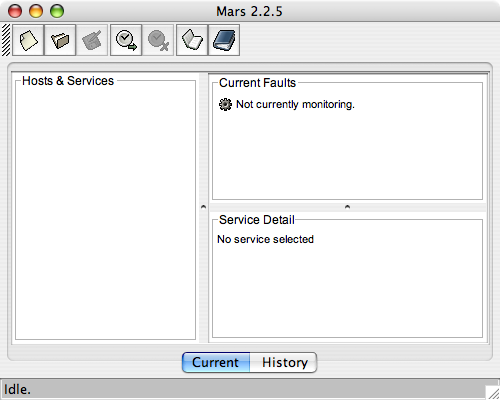
\includegraphics[scale=0.5]{images/screen_main_new}
\end{center}
\caption{The Mars main window with a new, empty configuration}
\label{fig_screen_main_new}
\end{figure*} 

To run Mars, run \filename{mars.jar} (for Java 1.4 or later) or
\filename{mars-j13.jar} (for Java 1.3), either by double-clicking on
it (in the Macintosh Finder or Windows Explorer) or by changing to the
Mars home directory and typing \cmdline{java -jar mars.jar}.

When running Mars from the command line, you can specify a
previously-saved Mars configuration file to open on startup. In
addition, the following command-line options are available:

\begin{description}
\item[\mbox{-}\mbox{-}home] specify a ``home'' directory from which to
  load extensions and the probe definitions file. Defaults to
  \filename{.} (the current working directory).
\item[\mbox{-}\mbox{-}nogui] start without the graphical user
  interface. This is useful for running the mail notification plugin
  or seeing status changes on the console. Requires a configuration
  file to be given.
\item[\mbox{-}\mbox{-}geom] start the graphical user interface with
  the specified geometry, expressed as width and height in pixels
  joined with an 'x', for example, '800x600'.
\end{description}

Example: to run Mars in \filename{/usr/mars/mars.jar}, loading plugins
from \filename{~/.mars/} and the configuration file
\filename{~/mars-config.xml} without starting the user interface,
type:

\cmdline{java -jar /usr/mars/mars.jar --nogui --home ~/.mars
  ~/mars-config.xml}

When Mars starts, the splash screen will appear momentarily, informing
you of any extensions it finds and loads on startup. The the main
window appears (see figure \ref{fig_screen_main_new}.  The Mars main
window has three parts: a host/service tree, a fault list, and a
service detail panel. The host/service tree displays the hosts and
services Mars knows about; when Mars is actively monitoring, it also
displays the status of each service. The fault list displays all
current problems with monitored services. The service detail display
shows relevant details about the service selected in the host/service
tree.

\section{Adding Hosts and Services}

The host/service tree can be manipulated in two ways: through a
context menu on the tree, or via keyboard commands.

By right-clicking (control-clicking on Macintosh) on a host or
service in the tree, or on blank space within the tree, you can bring
up the context menu, which allows you to access relevant tree editing
operations. Since you've started with a new configuration, the
host/service tree is empty; anywhere you right-click will bring up a
context menu with a single option, \guiitem{New Host...}. Select this
option to bring up a host editor on a new host.

\subsection{The Host Editor}
\begin{figure*}
\begin{center}
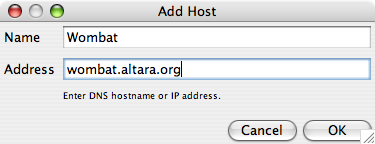
\includegraphics[scale=0.5]{images/screen_newhost}
\end{center}
\caption{The Mars host editor}
\label{fig_screen_newhost}
\end{figure*} 

The host editor (see figure \ref{fig_screen_newhost}) has two fields:

\begin{description}
\item[Name] is the name by which you want Mars to refer to the host;
  it could be the host name without the domain, or a descriptive name
  (e.g. ``Web Server'') completely unrelated to the host's actual DNS
  name.
\item[Address] is the fully qualified DNS name or IP address of the
  host.  Mars will perform a lookup of the given name before adding
  the host to the host/service tree, and will not allow you to
  continue unless the given name resolves to an address; this ensures
  you don't get false alarms about services being down because of a
  typo in the \guiitem{Address} field.
\end{description}	

\subsection{The Service Editor}
\begin{figure*}
\begin{center}
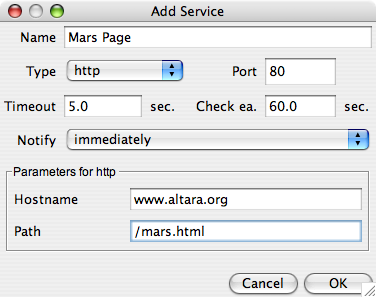
\includegraphics[scale=0.5]{images/screen_newsvc}
\end{center}
\caption{The Mars service editor}
\label{fig_screen_newsvc}
\end{figure*} 

Now that you've defined a host, you need to define a set of services
to monitor on that host. Right-click (control-click) on the host name
to bring up the host context menu and select \guiitem{Add Service...},
which will bring up a service editor on a new service on the selected
host.

The service editor (see figure \ref{fig_screen_newsvc} has the
following fields:

\begin{description}
\item[Name] is, as for a Host, simply a label by which Mars will
  display the service. Suggestions are the name of the service
  (``http''), the server software (``Tomcat''), or the user-visible
  application the service provides (``PR System'').
\item[Type] is the type of service -- Mars uses this to know how to
  probe a service. Currently, there are seven available service types
  (more services may be added by installing additional probe
  extensions):
\begin{description}
\item[http] probes HTTP/1.1 servers. It is useful for checking any web
  service.  Through its \guiitem{Hostname} parameter, you can specify
  the HTTP/1.1 \identifier{Host:} request header to send with each
  request. This is can be used to differentiate named virtual hosts
  during probing. The default hostname is the address of the host on
  which the service is running.  Through its \guiitem{Path} parameter,
  you can specify any path on the given server to monitor. The
  \guiitem{Path} is the portion of the URL after the host
  and port, starting with the first slash. The default path is
  \filename{/}.
\item[http-regex] probes HTTP/1.1 servers, but retrieves the body of
  the document along with the header, then tests the body against
  specified regular expressions for success and failure. If the
  failure expression matches in the body, the service will fail with
  status \identifier{bad reply}. If neither the success nor the
  failure expressions match in the body, the service will fail with
  status \identifier{closing}. Expressions left blank will not be
  matched.
\item[ftp] probes FTP servers.
\item[smtp] probes SMTP (Mail Transfer Agent) servers.
\item[imap] probes IMAPv4 servers.
\item[pop3] probes POP3 servers.
\item[ssh] probes Secure Shell servers (either version 1 or 2).
\item[tcp-connect] probes any TCP-based service for connection. {\em
  \guiitem{tcp-connect} does not test any protocol interaction; it
  only ensures that the host is accepting connections on the given
  port.} Use \guiitem{tcp-connect} to monitor services whose protocols
  Mars does not yet support, but understand that this service type is
  less reliable at detecting failure than the others.
\end{description}
\item[Port] is the TCP port on the host on which the service is
  running.  Each time you select a new \guiitem{Type}, this changes to
  the default port for the given service type.
\item[Timeout] is the time, in seconds, Mars will wait for a service
  to respond before considering it timed out. The default is 5.0
  seconds, but this may be far too long or far too short, depending on
  the service and your environment. If you notice a service that is up
  reporting back as timed out very often, consider increasing this
  value.
\item[Check ea. (n) sec.] is the minimum time Mars will delay between
  running probes of a service. Use longer delays here to decrease
  monitoring network traffic.
\item[Notify] determines how Mars will treat status change
  notifications for this service. Note that setting the notification
  behavior here {\em will not} have any effect unless you also enable
  at least one notification plugin (see section
  \ref{sec_extension}). The following notification behaviors are
  available:
\begin{description}
\item[never] causes Mars never to send notifications for this
  service. Use this for services whose status is not important enough
  for notification.
\item[immediately] causes Mars to send notifications immediately on
  any service status change. This is the default behavior, and the
  behavior of Mars versions prior to 2.2.2.
\item[on second attempt] causes Mars to wait for two consecutive
  probes to return the new status before notifying of the status
  change. Use this to prevent transient failures (e.g. timeout due to
  temporary network congestion) from triggering notifications.
\item[on third attempt] similarly waits for three consecutive
  probes. Use this to be even more aggressive about filtering out
  transient failures.
\end{description}
\item[Parameters for...] is a panel in which service-type specific
  parameters are set. Currently, only \guiitem{http} and
  \guiitem{http-regexp} use this panel.
\end{description}

Repeat this process until all the hosts and services you wish to
monitor with Mars have been added to the host/service tree. If you
have multiple hosts that have the same services, you can use the
\guiitem{Duplicate Host...} context menu item to create a new host
with the same services as an existing host.

Once you've finished configuring Mars, you'll probably want to save
your configuration; do this by selecting \guiitem{Save} from the
\guiitem{File} menu, clicking the save button on the toolbar, or
typing \keystroke{Ctrl-S} (\keystroke{Cmd-S} on Macintosh).

This will bring up a dialog asking you for the name of the file to
save the configuration into; the configuration will be written as an
XML file, the format of which is described in the {\sl Hacker's
  Guide}.

\subsection{Keyboard Editing}

The host/service tree can also be edited entirely with keyboard
commands, as follows:

\begin{description}
\item[up/down arrows] Select next or previous host or service.
\item[left arrow] Expand selected host, select first service.
\item[enter] Edit the selected host or service.
\item[delete] Delete the selected host or service.
\item[Ctrl-T/Cmd-T] Create a new host.
\item[Ctrl-R/Cmd-R] Create a new service on the selected host.
\item[Ctrl-D/Cmd-D] Duplicate the selected host.
\end{description}

\section{Monitoring Services with Mars}
\begin{figure*}
\begin{center}
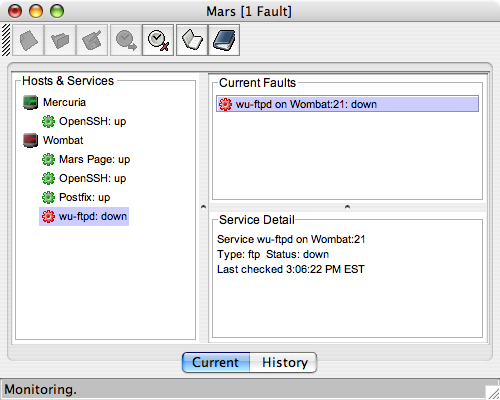
\includegraphics[scale=0.5]{images/screen_monitoring}
\end{center}
\caption{Mars in action}
\label{fig_screen_monitoring}
\end{figure*} 
\begin{figure*}
\begin{center}
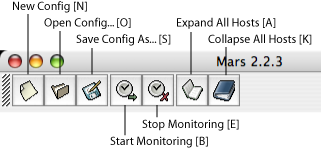
\includegraphics[scale=0.5]{images/screen_toolbar}
\end{center}
\caption{Mars toolbar}
\label{fig_screen_toolbar}
\end{figure*} 
\begin{figure*}
\begin{center}
\includegraphics[scale=0.5]{images/screen_menubars}
\end{center}
\caption{Mars menubars}
\label{fig_screen_menubars}
\end{figure*} 

To begin monitoring services with Mars, select \guiitem{Start} from
the \guiitem{Control} menu, click the start button in the toolbar, or
type \keystroke{Ctrl-B} (\keystroke{Cmd-B} on Macintosh).  Mars will
begin monitoring the services you have specified, display each
service's status in the host/service tree, and display any faults in
the fault list (see figure \ref{fig_screen_monitoring}).  While Mars
is actively monitoring, the number of faulted services appears in the
title bar. This allows you to minimize the Mars window and still keep
a summary eye on your network.
 
To see a host's services in the host/service tree, double-click on the
host's name or icon. To see detailed information for a service, click
on that service to select it; the detailed information will be
displayed in the service details pane. You can also click on a faulted
service in the fault list to see that service's details.

To fully expand the host/service tree, select \guiitem{Expand Hosts}
from the \guiitem{View} menu, click the expand button in the toolbar,
or type \keystroke{Ctrl-A} (\keystroke{Cmd-A} on Macintosh). To
collapse the tree (and view only hosts), select \guiitem{Collapse
  Hosts} from the \guiitem{View} menu, click the collapse button in
the toolbar, or type \keystroke{Ctrl-K} (\keystroke{Cmd-K} on
Macintosh).

A serice's status is expressed as one of the following:

\begin{description}
\item[down] The host is not accepting connections at the specified
  port. This generally means the service is not running, or the host
  is not connected to the network. This fault can also occur if there
  is a firewall between the host and the machine on on which Mars is
  running set to deny connections to the specified port. Check your
  firewall configuration to ensure the host is actually down.
\item[closing] The host is accepting connections at the specified
  port, but is closing the connection unexpectedly during the
  probe. This status is returned for \guiitem{http-regexp} services
  when neither the success nor failure expressions match. Another
  common cause of this is services wrapped with tcpd, or other
  IP-address based access control software, set to deny connections
  from the machine on which Mars is running.  Check your wrappers
  configuration; if connections should be allowed from the machine on
  which Mars is running, there is something wrong with the service.
\item[bad reply] The service is returning unexpected data during the
  probe.  The service may or may not be down; check the ``Received''
  line in the service details pane to see what the service
  returned. For \guiitem{http} services, this means the server
  returned an error result code (4xx or 5xx).
\item[timeout] The service is not giving an expected response during
  the specified timeout period. This may indicate excessive load on
  the service. If you see this fault often, and the service is
  operating properly, consider increasing the timeout delay for the
  service.
\item[up] The service is operating properly, and responding within the
  specified timeout.
\item[probe error] An unspecified Mars error occurred during the probe
  of the service. This may occur during shutdown, or as the result of
  a bug in Mars itself.
\item[unknown] The service has not been probed since Mars started, or
  since it was first added. Wait a moment for the probe to finish
  running.
\end{description}

If a host has no faulted services, its icon appears green in the
host/service tree while Mars is monitoring. If any of a host's
services are faulted, that host's icon will appear red.

If you'd like to ignore a fault but keep monitoring the service, you
may hide that fault by right-clicking in the fault list and selecting
\guiitem{Hide} from the menu that appears. The service is still being
monitored; it's just hidden in the fault list. Hidden faults may be
shown via the \guiitem{Show All} menu item.

The history of each service's status is displayed in the recent
changes list.  The recent changes list is accessible via the
\guiitem{History} tab in the Mars window.  This list shows the 200
most recent service status changes, and can be cleared using the
\guiitem{Clear History} button.

To stop Mars from monitoring, select \guiitem{Stop} from the
\guiitem{Control} menu, click the stop button in the toolbar, or type
\keystroke{Ctrl-E} (\keystroke{Cmd-E} on Macintosh). You'll notice
when Mars is stopped, all current faults disappear from the fault
list, and the host/service tree reverts to showing no status for each
service.

\section{Plugins and Probe Extensions}
\label{sec_extension}

Mars supports plugins, independent modules of Java code that can
listen for service status changes and act upon them
accordingly. Plugins are dynamically loaded from the Mars home
directory at startup time, and are listed and configured via the
\guiitem {Plugins} menu.  Plugins are shipped in the \filename{extras}
directory in the Mars distribution, and will need to be moved to the
home directory in order to load at startup time.

Mars also supports probe extensions, dynamically loaded Java classes
which add new service monitoring capabilities to Mars. Probe
extensions are shipped in the \filename{extras} directory within the
Mars distribution; you'll need to move them to the Mars home directory
in order for them to load at startup time. Each of these probe
extensions adds a service type to the available services Mars can
probe.

\subsection{UI Notification}

The UI Notification plugin displays a dialog box when certain service
status changes occur. To install UI Notification, move
\filename{plugin\_swingnotify.jar} from the \filename{extras}
directory into your Mars home directory.

To enable UI notification, select it in the
\guiitem{Plugins} menu; the UI notification editor will pop up. Select
the \guiitem{Enabled} checkbox to enable notification. Select
\guiitem{Beep on fault} to cause Mars to beep when displaying a
notification. The \guiitem{Notify when a service comes back up}
checkbox causes Mars to display another dialog when a service comes
back up.

UI Notification requires the Swing user interface, and will be
disabled if the \identifier{\mbox{-}\mbox{-}nogui} command-line option
is in effect.

\subsection{Mail Notification}

This plugin uses a very simple SMTP client to send a very simple
message to a given list of e-mail addresses using a single given mail
server whenever a service is detected as faulted. To install Mail
Notification, move \filename{plugin\_mailnotify.jar} from the
\filename{extras} directory into your Mars home directory.

To enable Mail Notification, select it in the \guiitem{Plugins} menu;
the mail notification editor will pop up. Select the \guiitem{Enabled}
checkbox to enable notification, then fill in the \guiitem{SMTP
  Server} field with the address or DNS hostname of a SMTP server
configured to relay mail from the machine on which Mars is running.

To specify a set of recipients for the notification e-mail, enter the
addresses into the \guiitem{Recipient(s)} field separated by commas,
as you would in most popular mail client programs.  To specify a
``From'' address to appear on each notification e-mail, place the
address in the \guiitem{Sender} field. If you leave this field blank,
it will default to the first address in the recipient list. Note that
the addresses in these fields must be of the form
\identifier{host@subdomain.domain.dom} only; you must omit angle
brackets, or proper names, quoted or not.

As with the UI Notification plugin, the \guiitem{Notify when a service
  comes back up} checkbox causes Mars to send another message when a
service comes back up.

With the Mail Notification plugin enabled, you can run Mars
``headless'' -- i.e., without a GUI. To do this, first run Mars to
create a configuration file with the hosts and services you wish to
monitor, and with Mail Notification configured and enabled. Save this
config file, then invoke Mars from the command line with the
\cmdline{--nogui} option. Mars will print status messages to the
console and send email notifications when services go down or time
out.

\subsection{CSV Logger}

This plugin logs the results of each probe to a CSV (comma-separated
values) file, in the following format: \identifier{date, time,
  host-name, service-name, host-address, port, service-type, status,
  response-time}. The date and time are given in ISO-8601 format
(\identifier{year/mo/dy hr:mn:sc.msc}) Response time is given in
milliseconds. To install CSV logging, move
\filename{plugin\_csvlog.jar} from the \filename{extras}
directory into your Mars home directory.

To enable CSV logging, select it in the \guiitem{Plugins} menu; the
CSV logging editor will pop up. Select the \guiitem{Enabled} checkbox
to enable logging, then fill in a pathname to a CSV file to log to in
the \guiitem{Log file} field. You can use the \guiitem{Choose...}
button to select a pathname using the file browser, if you like. The
selected log file path must be within an existing directory and
writable by you.

If the given log file exists, the CSV Logger plugin will append new
CSV log entries to the end of it. This means you can log probe
information across multiple runs of Mars without having to reconfigure
the CSV Logger or lose the old data each time.

With the CVS Logger plugin enabled, you can run Mars ``headless'' --
i.e., without a GUI. To do this, first run Mars to create a
configuration file with the hosts and services you wish to monitor,
and with the logger configured and enabled. Save this config file,
then invoke Mars from the command line with the \cmdline{--nogui}
option. Mars will print status messages to the console and write a log
to the specified logfile.

\subsection{XML Snapshot}

This plugin periodically dumps status information on the services Mars
is monitoring into a named XML file. This XML file has the same format
as the Mars configuration file (see the Hacker's Guide for more), but
with status information in the \identifier{status} element within each
\identifier{service}. This plugin is designed to be used with XSL
transformations to display status information from Mars via a web
interface. To install the XML Snapshot plugin, move
\filename{plugin\_xmlsnap.jar} from the \filename{extras} directory
into your Mars home directory.

To enable the XML Snapshot plugin, select it in the \guiitem{Plugins}
menu; the XML Snapshot editor will pop up. Select the
\guiitem{Enabled} checkbox to enable logging, then fill in a pathname
to an XML file to dump to in the \guiitem{XML file} field. You can use
the \guiitem{Choose...}  button to select a pathname using the file
browser, if you like. The selected path must be within an
existing directory and writable by you.

XML snapshots are written every 60 seconds by default; to change this,
enter a new time in the \guiitem{Period} field.

With the XML Snapshot plugin enabled, you can run Mars ``headless'' --
i.e., without a GUI. To do this, first run Mars to create a
configuration file with the hosts and services you wish to monitor,
and with the logger configured and enabled. Save this config file,
then invoke Mars from the command line with the \cmdline{--nogui}
option. Mars will print status messages to the console and dump status
information to the specified snapshot file.

\subsection{XMPP Notification}

This plugin sends notification via an XMPP (Jabber) instant-messaging
server whenever a service is detected as faulted.  The XMPP
Notification plugin includes the Smack XMPP client library version
1.2.1, \copyright 2002-2003 Jive Software, Inc., all rights
reserved. Smack is developed by Jive Software, and is available at
\url{http://www.jivesoftware.com/xmpp/smack}. To install XMPP
notification, move \filename{plugin\_xmpp.jar} from the
\filename{extras} directory into your Mars home directory.

To enable XMPP notification, select it in the \guiitem{Plugins} menu;
the XMPP notification editor will pop up. Select the \guiitem{Enabled}
checkbox to enable notification, then fill in the form. \guiitem{XMPP
  Server} and \guiitem{XMPP Port} identify the server to connect to
use to send notification messages.  \guiitem{Username} and
\guiitem{Password} are the credentials used to connect to the
server. The string in \guiitem{Prefix} will be appended to each
message sent by the plugin. \guiitem{Recipient(s)} is a list of Jabber
addresses to send the notification to. Separate multiple addresses
with commas.

With the XMPP Notification plugin enabled, you can run Mars
``headless'' -- i.e., without a GUI. To do this, first run Mars to
create a configuration file with the hosts and services you wish to
monitor, and with the plugin configured and enabled. Save this config
file, then invoke Mars from the command line with the
\cmdline{--nogui} option. Mars will print status messages to the
console and send notifications via XMPP.

\subsection{Client Debugger}

This plugin provides a detailed view of Mars' interaction with remote
hosts in real time. It is intended for debugging XML-defined probes in
\filename{mars-def.xml} and probe extensions.  To install the client
debugger, move \filename{plugin\_cdebug.jar} from the
\filename{extras} directory into your Mars home directory.

To use the client debugger, select it in the \guiitem{Plugins} menu;
the client debugger preferences will pop up. Select the
\guiitem{Enabled} checkbox and set the \guiitem{Horizon} slider to the
number of sessions you want the debugger to remember.

A new tab, \guiitem{Debug}, will appear in the Mars window. This tab
is split into two panels, a debug session list and a session detail
display. Debug sessions are displayed by timestamp (most recent
first), the name of the client interface producing them and some
identifying information about the connection. XML-defined probes (and
the Mars mail notification client) are implemented by a class called
\identifier{SendExpectClient}, so these sessions are defined by the
client interface \identifier{SEC}. The included HTTPS and JDBC probe
extensions are identified, respectively, as \identifier{HTTPS} and
\identifier{JDBC}.

By selecting a session in the upper panel, the session's details will
appear in the lower panel. There are three types of entries in a
session: data sent (green right double arrow), data recieved (yellow
left double arrow), and information (``i'' in a blue circle). Sent and
received data is split into lines; the special symbols
\identifier{<CR>} and \identifier{<LF>} are used for carriage return
and linefeed. The timestamp on each entry is the time of the
sending/receipt of the first character in the entry.

The Client Debugger requires the Swing user interface, and will be
disabled if the \identifier{\mbox{-}\mbox{-}nogui} command-line option
is in effect.

\subsection{Mac OS X Integration}

This plugin is provides integration between Mars and the Mac OS X
environment. It is primarily intended for use by the
\filename{Mars.app} Mac OS X application-bundle version of Mars, and
is not included with the non-Macintosh binary distribution. See the
section \ref{sec_macosx} for more.

\subsection{HTTPS Probe Extension}

This probe extension adds a new service type, https, to the available
service types, which probes secure HTTP servers.  To install the HTTPS
probe extension, move \filename{probe\_https.jar} from the
\filename{extras} directory into your Mars home directory.

The https service takes three parameters. \guiitem{Hostname} and
\guiitem{Path} are used as they are with the other http
services. \guiitem{Content}, if present, is a plain text string to
scan for in the response body. It is {\em not} the same as the regular
expressions supported by the http-regexp

Note that the https service appears to report failure for any server
presenting a certificate not signed by a certificate authority in the
\filename{lib/security/cacerts} file in your Java installation. Use
the \identifier{keytool} program included with Java to modify this
file.

\subsection{JDBC Probe Extension}

This probe extension adds a new service type, jdbc, to the available
service types, which probes JDBC-accessible database servers. To
install the JDBC probe extension, move \filename{probe\_jdbc.jar} from
the \filename{extras} directory into your Mars home directory.

The jdbc service takes five parameters. \guiitem{Protocol} is the
database protocol to use (the protocol part after \identifier{jdbc:} in a
JDBC URL). \guiitem{Driver} is the name of the Java class of the JDBC
driver to use. This driver must be in the system classpath at Mars
startup time to be usable by the JDBC probe. \guiitem[Database] is the
name of the database to connect to, and \guiitem[Username] and
\guiitem[Password] are the credentials to present.

\section{Mars on Mac OS X}
\label{sec_macosx}

A version of Mars built to take advantage of Mac OS X's support for
Java applications is available separately as a \filename{.dmg} disk
image file. This disk image contains a Mac OS X installer package
which will place a Mac-friendly Mars in your
\filename{Applications} directory. This manual applies in full to the
Mac OS X version of Mars with a few caveats:

\begin{itemize}
\item Mars for Mac OS X requires Java 1.4. You can run the
  non-Macintosh version of Mars on Java 1.3, but it won't integrate
  nicely with Mac OS X.
\item Mars can be started simply by double-clicking the application in
  \filename{Applications}.
\item The Mars home directory is contained in
  \filename{/Library/Leapfrog/Mars}. To install Mars extensions,
  you'll need to place them in that directory. All included extensions
  are already installed by the Mars installer package.
\item To open configuration files from the command line, use
  \cmdline{open -a Mars}.
\end{itemize}

The Mac-friendly version of Mars provides several benefits, as follows: 

\begin{itemize}
\item The Mars menu bar appears at the top of the screen, as with
  other Macintosh applications, and not in the window as with the
  non-Macintosh version.
\item The Mars window's close box (``jellybean?'') will display the
  ``dirty'' dot if the configuration has been changed since the last
  save.
\item The \guiitem{Quit} item on the application menu works properly;
  with the non-Macintosh version, this menu item will always quit
  without asking whether any unsaved changes should be saved. 
\item The \guiitem{About Mars...} item on the Application menu will
  re-display the Mars splash screen.
\item Mac-friendly Mars has a pretty (or at least identifiable) dock icon.
\item Mars' dock icon will accept drag-and-drop of XML files for use
  as configuration files.
\end{itemize}

\appendix
\section{Change History}
\subsection{Mars 2.2.7 -- March 22, 2004}
Mars 2.2.7 is a bugfix release. The following changes were made:
\begin{itemize}
\item SimpleSmtpClient (used in the mail notification plugin) now
  properly uses CR/LF to terminate lines sent to the mail
  server. This, like the bug fixed in 2.2.3 in the probe engine, was
  not technically RFC-compliant, and was causing problems with mail
  notification on Microsoft servers. Thanks to Sebastian Johnck and
  Aaron Roller for their help with this bug.
\item Bugfixes to JDBC Probe and tcp-connect service types, thanks to
  S. \c Ca\u glar Onur.
\item XMPP notification now properly handles multiple recipients,
  thanks to a fix submitted by Paul Goulbourn.
\end{itemize}

\subsection{Mars 2.2.6 -- March 1, 2004}
Mars 2.2.6 is a feature enhancement and bugfix release. The following
changes were made:
\begin{itemize}
\item Plugins may now display their own tabs in the Mars main
  window. This functionality is intended for the construction of data
  visualization plugins, and is used by the new Mars Client Debugger.
\item A new Client Debugger plugin has been added. This allows users
  to view all Mars' interactions with the network, in real time, and
  is primarily intended to aid in the development of new probe
  extensions and XML-based probes.
\item All included probe extensions and plugins have been instrumented
  to report to the client debugger.
\item All included probe extensions and plugins are now distributed in
  the \filename{extras} directory.
\item Timestamps have been added to console status messages in
  \identifier{\mbox{-}\mbox{-}nogui} mode.
\item The service detail view now displays the next scheduled probe time.
\item Plugins that use the user interface will now refuse to load in
  \identifier{\mbox{-}\mbox{-}nogui} mode.
\item A new XML Snapshot plugin has been added. Thanks to Robert
  Fuller for working on this.
\item A minor bug which occasionally caused the \guiitem{received}
  property of XML-defined probes to be corrupted with an internal
  end-of-stream marker has been fixed.
\item Mars now explicitly uses UTF8 encoding for its configuration
  file.
\end{itemize}

\subsection{Mars 2.2.5 -- February 10, 2004}
Mars 2.2.5 is a bugfix and feature enhancement release. The following
changes were made:
\begin{itemize}
\item Loading configuration files from the command line works
  again. This was, officially, a Really Embarrasing Bug.
\item XMPP notification bugfixes. XMPP client connection is now
  properly stopped on disable, and restarted on configuration
  change. Thanks to Mike Dixson for his help in tracking this down.
\item Tweaked open/save dialogs to actually change to the correct
  directory on all platforms. Default to saving new configuration
  files in home directory. Fixed minor bugs in configuration file
  handling.
\item Mars' user interface has undergone a minor overhaul. Mars now
  has a menu bar. The host/service tree is editable using the
  keyboard. The Config panel has been replaced by the Plugins menu.
\item Mac OS X integration is Mac-friendlier. Mars now uses the system
  menubar and the ``dirty'' dot in the close jellybean. Configuration
  file open through the Finder now works properly even if Mars wasn't
  running yet. Oops.
\end{itemize}

\subsection{Mars 2.2.4 -- February 4, 2004}
Mars 2.2.4 is a feature enhancement and bugfix release. The following
changes were made:
\begin{itemize}
\item JDBC is now supported by an included probe extension, thanks to
  Jon Steele.
\item Notification via XMPP (Jabber) is now supported by an included
  plugin, thanks to Robert Fuller.
\item Mars now integrates with Mac OS X (Java 1.4 or greater) via an
  included plugin. Mars is now additionally distributed as a
  ``native'' Mac OS X application.
\item Tweaked client code to put packets on the wire only when a send
  was completed; previously, Mars would send many unnecessarily small
  TCP segments when probing, especially HTTP and its ilk. While this
  behavior was not technically incorrect, it could theoretically cause
  problems with some poorly coded servers, and was (ever so slightly)
  disrespectful of the network.
\end{itemize}

\subsection{Mars 2.2.3 -- January 26, 2004}
Mars 2.2.3 is a feature enhancement and bugfix release. The following
requests have been addressed:
\begin{description}
\item[611897] HTTPS is now supported by an included probe extension,
  thanks to Scott Ahten.
\item[726603] Added expand and collapse toolbar buttons, for quicker
  access to the host/service tree, at the suggestion of Richard Gill.
\item[838540] Fixed bug that would cause Mars to send LF where CRLF is
  required. Apparently, most (Unix-based) services don't really care
  about the CR. This should fix up problems on probing certain
  Windows-based services. Thank you, Noel Bergman.
\item[851943] Changed all date output to conform to ISO 8601.
\item[851944] Added ability to reference a regular expression
  contained in a service parameter, and the http-regexp service to
  take advantage of this. Thanks to Robert Fuller.
\item[851945] Added the ability to specify the geometry of the Mars
  window on the command line, at the suggestion of Stefan Svensson.
\item[851946] Added code to extension loader to allow multiple plugins
  to reside in the same .jar file. This is not presently used by the
  shipping Mars system, but could be used by plugin/probe developers
  to avoid clutter in the Mars home directory. Thank you, Ivica
  Loncar.
\end{description}

\subsection{Mars 2.2.2 -- March 11, 2003}
Mars 2.2.2 is a feature enhancement and bugfix release. The following requests
have been addressed:
\begin{description}
\item[590319] Added host icon coloring according to service status.
\item[590333] Added CSV Logger plugin
\item[631869] Added ability to choose notification retry count by service.
Added \identifier{NotificationListener} interface to plugin framework and
\identifier{Notifier} class to engine to support delayed notification.
\item[683792] Fixed mail notification bug that caused problems with some SMTP
servers which require MAIL and RCPT addresses to be enclosed in angle brackets.
Thanks to Laurent Marot for helping me track this one down.
\item[692534] Added ability to send notifications to multiple e-mail recipients.
\item[693452] Fixed bug that would cause the information in the status bar to
fall behind the monitoring engine when Mars is very busy.
\item[693456] Added \guiitem{Hostname to Monitor} parameter to HTTP probe.
Added \identifier{\%\%(remote-hostname)} parameter hack to
\filename{mars-def.xml} to support this.
\item[700452] Updated Jakarta ORO and Xerces-J packages.
\end{description}

\subsection{Mars 2.2.1 -- February 25, 2003}
Mars 2.2.1 is a feature enhancement and bugfix release. The following requests
have been addressed:
\begin{description}
\item[590325] Added a status bar.
\item[590328] Added dynamic loading of plugins and probe extensions.
\item[632639] The UI Notification plugin now runs in a separate thread, to keep
from blocking other status change notifications. Thanks to Mark Lewis for
sending in this patch.
\item[629689] The Mail Notification plugin now allows mail to be sent from a
different address than the recipient address. Thanks to Mark Lewis for sending
in this patch.
\end{description}

\subsection{Mars 2.2.0 -- October 28, 2002}
Mars 2.2.0 is an under-the-hood feature enhancement and bugfix release. The
following requests have been addressed:
\begin{description}
\item[594660] Added the ability to define probes using XML.
\item[602762] Fixed a bug in SMTP probing which was looking for an incorrect
response from SMTP servers.
\end{description}

\subsection{Mars 2.1.3 -- August 12, 2002}
Mars 2.1.3 is a feature enhancement release. The following features have been
added:
\begin{description}
\item[590315] Added the ability to hide faults in the fault list.
\item[590316] Added the ability to clear the status history.
\item[590323] Added the Duplicate Host... command to the service tree context
menu, which makes a copy of a given host with a different name and address.
\item[590330] Added the ability to send a notification when a service comes
back up to the mail notification plugin.
\item[593098] Bound the selection in the fault list to the service tree, so
that when the user clicks on a fault in the fault list, that service is
selected in the service tree (which also causes it to be displayed in the
detail display).
\end{description}

\subsection{Mars 2.1.2 -- July 14, 2002}
Mars 2.1.2 is a bugfix/feature enhancement release.  Fixed in this release is
the bug/misfeature that forced the user to stop monitoring before editing the
host/service tree - hosts and services can now be added, edited, or deleted at
any time. Also added is the ability to specify a path to an HTTP probe; now you
can use Mars to check to make sure your web applications and services are
running properly (i.e. not replying 500 Server Error, which will show up as a
``bad reply'' in Mars) - not just to check that your web server itself is
running.

\subsection{Mars 2.1.1 -- June 30, 2002}
Mars 2.1.1 is a bugfix release. Fixed in this release are a bug in the probe
client that caused all sorts of problems on Win2k (namely a CPU usage spike and
an enormous memory leak), and a minor design flaw in the HTTP probe. Formerly,
an HTTP server had to respond to the probe with a 200 (OK) response status to
be considered ``up''; valid ``up'' responses such as the 3xx redirect codes were
shown as ``timed out''. No new features were added in this release.

\subsection{Mars 2.1.0 -- June 5, 2002}
Mars 2.1.0 is a bugfix/feature enhancement release.  The user interface and
functionality is largely the same. In addition to various user interface tweaks
and bug fixes, Mars 2.1.0 features:
\begin{itemize}
\item A rewritten probe client backend that fixes a couple of rather
embarrassing bugs that can cause Mars to hang.  This rewritten backend properly
handles services that accept connections then fail to respond without hanging
Mars. It's also more flexible, and may be used in the future to allow simple
TCP/IP text based probes to be described in XML.
\item A properly multithreaded probing engine. Though Mars 2.0.0 was designed
to support multiple probe threads running at once, only one probe thread was
used for simplicity. The probe engine now properly starts the correct number of
threads to ensure that ``probe each n sec.'' parameters on services are met,
within reason.
\item Support for a plugin framework, though planned autoload of plugins from
.jar files has not yet been written (autoload is supported in Mars 2.2.1). A
plugin for notifying of service faults via email was added, as well.  
\end{itemize}

\subsection{Mars 2.0.0 -- May 8, 2002}
Mars 2 is a complete rewrite of Mars. The first and most noticeable change is
that the user interface is completely different. The second is that the
configuration file format is completely different.  In addition, several Mars
1.x features have been removed, including:
\begin{itemize}
\item SPOTS. Mars can no longer talk to the SPOTS agent, which provides load
average, memory usage, and filesystem usage information on Unix systems. SPOTS
is inconsistent with a strictly services-oriented view of a host, though I may
add some sort of agent support like SPOTS in future versions if enough of you
really miss it.
\item Notification of down services, via the GUI and email. (Notification is
supported in Mars 2.1.0.)
\end{itemize}
\end{document}
